\lab{Facial Recognition}{Facial Recognition}
\label{lab:FacialRecognition}

\objective{
A \emph{facial recognition} algorithm attempts to match a person's portrait to a database of many portraits.
Facial recognition is becoming increasingly important in security, law enforcement, artificial intelligence, and other areas.
Though humans can easily match pictures to people, computers are beginning to surpass humans at facial recognition.
In this lab, we implement a basic facial recognition system that relies on eigenvectors and the SVD to efficiently determine the difference between faces.
}

\section*{Preparing an Image Database} % ======================================

The \texttt{faces94} face image dataset\footnote{See \url{http://cswww.essex.ac.uk/mv/allfaces/faces94.html}.} contains several photographs of 153 people, organized into folders by person.
To perform facial recognition on this dataset, select one image per person and convert these images into a database.
For this particular facial recognition algorithm, the entire database can be stored in just a few NumPy arrays.

Digital images are stored on computers as arrays of pixels.
Therefore, an $m \times n$ image can be stored in memory as an $m\times n$ matrix or, equivalently, as an $mn$-vector by concatenating the rows of the matrix.
Then a collection of $k$ images can be stored as a single $mn\times k$ matrix $F$, where each column of $F$ represents a single image.
That is, if
\[
F = \left[\begin{array}{c|c|c|c}
\arrayrulecolor{lightgray}
& & & \\
\f_1 & \f_2 & \cdots & \f_k
\\
& & &
\end{array}\right],
\]
then each $\f_i$ is a $mn$-vector representing a single image.

The following function obtains one image for each person in the \texttt{faces94} dataset and converts the collection of images into an $mn \times k$ matrix $F$ described above.

\begin{lstlisting}
import numpy as np
from os import walk
from scipy.misc import imread

def get_faces(path="./faces94"):
    # Traverse the directory and get one image per subdirectory.
    faces = []
    for (dirpath, dirnames, filenames) in walk(path):
        for fname in filenames:
            if fname[-3:]=="jpg":       # Only get jpg images.
                # Load the image, convert it to grayscale,
                # and flatten it into a vector.
                faces.append(np.ravel(imread(dirpath+"/"+fname, flatten=True)))
                break
    # Put all the face vectors column-wise into a matrix.
    return np.transpose(faces)
\end{lstlisting}

\begin{problem} % show_face() function.
Write a function that accepts an image as a flattened $mn$-vector, along with its original dimensions $m$ and $n$.
Use \li{np.reshape()} to convert the flattened image into its original $m\times n$ shape and display the result with \li{plt.imshow()}.
\\ (Hint: use \li{cmap='gray'} in \li{plt.imshow()} to display images in grayscale.)

Unzip the \texttt{faces94.zip} archive and use \li{get_faces()} to construct $F$.
Each \texttt{faces94} image is $200 \times 180$, and there are $153$ people in the dataset, so $F$ should be $36000 \times 153$.
Use your function to display one of the images stored in $F$.
\label{prob:visualize-faces}
\end{problem}

\section*{The Eigenfaces Method} % ============================================

With the image database $F$, we could construct a simple facial recognition system with the following strategy.
Let $\g$ be an $mn$-vector representing an unknown face that is not part of the database $F$.
Then the $\f_i$ that minimizes $\|\g - \f_i\|_2$ is the matching face.
Unfortunately, computing $\|\g - \f_i\|_2$ for each $i$ is very computationally expensive, especially if the images are high-resolution and/or the database contains a large number of images.
The \emph{eigenfaces method} is a way to reduce the computational cost of finding the closest matching face by focusing on only the most important features of each face.
Because the method ignores less significant facial features, it is also usually more accurate than the na\"ive method.

The first step of the algorithm is to shift the images by the \emph{mean face}.
Shifting a set of data by the mean exaggerates the distinguishing features of each entry.
In the context of facial recognition, shifting by the mean accentuates the unique features of each face.
For the images vectors stored in $F$, the mean face $\boldsymbol{\mu}$ is the defined to be the element-wise average of the $\f_i$.
\[
\boldsymbol{\mu} = \frac{1}{k}\sum_{i=1}^k \f_i
\]
Hence, the $i$th mean-shifted face vector $\bar{\f}_i$ is given by
\[
\bar{\f}_i = \f_i - \boldsymbol{\mu}.
\]
Next, define $\bar{F}$ as the $mn \times k$ matrix whose columns are given by the mean-shifted face vectors:
\[
\bar{F} = \left[\begin{array}{c|c|c|c}
\arrayrulecolor{lightgray}
& & & \\
\bar{\f}_1 & \bar{\f}_2 & \cdots & \bar{\f}_k
\\
& & &
\end{array}\right].
\]

\begin{figure}[H] % Mean face + shifted faces.
\captionsetup[subfigure]{justification=centering}
\centering
\begin{subfigure}{.32\textwidth}
    \centering
    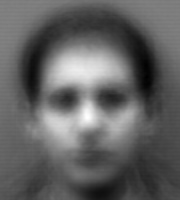
\includegraphics[width=\textwidth]{figures/meanFace.png}
    \caption{The mean face.}
    \label{fig:facerec-meanface}
\end{subfigure}
%
\begin{subfigure}{.32\textwidth}
    \centering
    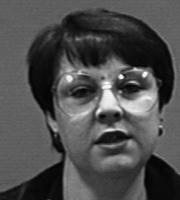
\includegraphics[width=\textwidth]{figures/originalFace0.png}
    \caption{An original face.}
    \label{fig:facerec-original}
\end{subfigure}
%
\begin{subfigure}{.32\textwidth}
    \centering
    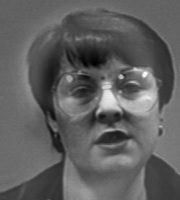
\includegraphics[width=\textwidth]{figures/differenceFace0.png}
    \caption{A mean-shifted face.}
    \label{fig:facerec-shifted}
\end{subfigure}
\caption{}
\end{figure}

\begin{problem} % Shift by the mean.
\label{prob:meanFace}
Write a class called \li{FacialRec} whose constructor accepts a path to a directory of images.
In the constructor, use \li{get_faces()} to construct $F$, then compute the mean face $\boldsymbol\mu$ and the shifted faces $\bar{F}$.
Store each array as an attribute.
\\(Hint: Both $\boldsymbol\mu$ and $\bar{F}$ can be computed in a single line of code by using NumPy functions and/or array broadcasting.)

Use your function from Problem \ref{prob:visualize-faces} to visualize the mean face, and compare it to Figure \ref{fig:facerec-meanface}.
Also display an original face and its corresponding mean-shifted face.
Compare your results with Figures \ref{fig:facerec-original} and \ref{fig:facerec-shifted}.
\end{problem}

To increase computational efficiency and minimize storage, the face vectors can be represented with fewer values by projecting $\bar{F}$ onto a lower-dimensional subspace.
Let $s$ be a natural number such that $s < r$, where $r$ is the rank of $\bar{F}$.
By projecting $\bar{F}$ onto an $s$-dimensional subspace, each face can be stored with only $s$ values.

Specifically, let $U \Sigma V\hrm$ be the compact SVD of $\bar{F}$ with rank $r$, which can also be represented by
 \[
\bar{F}= \sum_{i=1}^r \sigma_i\u_i\v_i\hrm.
\]
The first $r$ columns of $U$ form a basis for the range of $\bar{F}$.
Recall that the Schmidt, Mirsky, Eckart-Young Theorem states that the matrix
\[
\bar{F}_s = \sum_{i=1}^s \sigma_i\u_i\v_i\hrm
\]
is the best rank-$s$ approximation of $\bar{F}$ for each $s < r$.
This means that $\| \bar{F} - \bar{F_s} \|$ is minimized against all other $\| \bar{F} - B \|$ where $B$ has rank $s$.
As a consequence of this theorem, the first $s$ columns of $U$ form a basis that provides the ``best'' $s$-dimensional subspace for approximating $\bar{F}$.

The $s$ basis vectors $\u_1, \ldots, \u_s$ are are commonly called the \emph{eigenfaces} because they are eigenvectors of $\bar{F}\bar{F}\trp$ and because they resemble face images.
Each original face image can be efficiently represented in terms of these eigenfaces.
See Figure \ref{fig:facerec-eigenfaces} for visualizations of the some of the eigenfaces for the \texttt{facesd94} data set.

\begin{figure}[H] % Eigenfaces.
\centering
\begin{subfigure}{.32\textwidth}
    \centering
    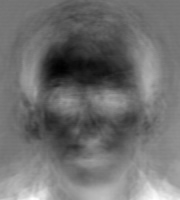
\includegraphics[width=\textwidth]{figures/eigenface0.png}
\end{subfigure}
%
\begin{subfigure}{.32\textwidth}
    \centering
    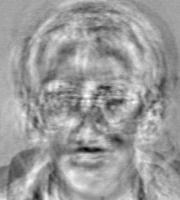
\includegraphics[width=\textwidth]{figures/eigenface49.png}
\end{subfigure}
%
\begin{subfigure}{.32\textwidth}
    \centering
    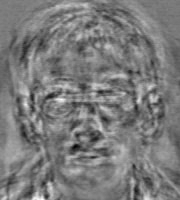
\includegraphics[width=\textwidth]{figures/eigenface99.png}
\end{subfigure}
\caption{The first, 50th, and 100th eigenfaces.}
\label{fig:facerec-eigenfaces}
\end{figure}

In general, the lower eigenfaces provide a more general information of a face and higher-ordered eigenfaces provide the details necessary to distinguish particular faces.%
\footnote{Neil Muller, Lourenco Magaia, and B. M. Herbst. \textit{Singular Value Decomposition, Eigenfaces, and 3D Reconstructions}. SIAM Review. 2004. 46:3, 518-545.}
These eigenfaces will be used to construct the face images in the dataset.
The more eigenfaces used, the more detailed the resulting image will be.

Next, let $U_s$ be the matrix with the first $s$ eigenfaces as columns.
Since the eigenfaces $\{\u_i\}_{i=1}^s$ form an orthonormal set, $U_s$ is an orthonormal matrix (independent of $s$) and hence $U_s\trp U_s = I$.
The matrix $P_s = U_sU_s\trp$ projects vectors in $\mathbb{R}^{mn}$ to the subspace spanned by the orthonormal basis $\{\u_i\}_{i=1}^s$, and the change of basis matrix $U_s\trp$ puts the projection in terms of the basis of eigenfaces.
Thus the projection $\widehat{\f}_i$ of $\bar{\f}_i$ in terms of the basis of eigenfaces is given by
%
\begin{equation}
\widehat{\f}_i = U_s\trp P_s\bar{\f}_i = U_s\trp U_s U_s\trp \bar{\f}_i = U_s\trp\bar{\f}_i.
\label{eq:facialrec-projection}
\end{equation}
%
Note carefully that though the shifted image $\bar{\f_i}$ has $mn$ entries, the projection $\widehat{\f}_i$ has only $s$ entries since $U_s$ is $mn\times s$.
Likewise, the matrix $\widehat{F}$ that has the projections $\widehat{\f}_i$ as columns is $s \times k$, and
\begin{equation}
\widehat{F} = U_s\trp F.
\label{eq:facialrec-projectall}
\end{equation}

\begin{problem} % Compute U, implement project().
In the constructor of \li{FacialRec}, calculate the compact SVD of $\bar{F}$ and save the matrix $U$ as an attribute.
Compare the computed eigenfaces (the columns of $U$) to Figure \ref{fig:facerec-eigenfaces}.

Also write a method that accepts a vector of length $mn$ or an $mn\times l$ matrix, as well as an integer $s$.
Construct $U_s$ by taking the first $s$ columns of $U$, then use (\ref{eq:facialrec-projection}) or (\ref{eq:facialrec-projectall}) to calculate the projection of the input vector or matrix onto the span of the first $s$ eigenfaces.
\\(Hint: this method should be implemented with a single line of code.)
\label{prob:facialrec-project}
\end{problem}

Reducing the mean-shifted face image $\bar{\f}_i$ to the lower-dimensional projection $\widehat{\f}_i$ drastically reduces the computational cost of the facial recognition algorithm, but this efficiency gain comes at a price.
A projection image only approximates the corresponding original image, but as long as $s$ isn't too small, the approximation is usually good enough for the algorithm to work well.
Before completing the facial recognition system, we reconstruct some of these projections to visualize the amount of information lost.

From (\ref{eq:facialrec-projection}), since $U_s\trp$ projects $\bar{\f}_i$ and performs a change of basis to get $\widehat{\f}_i$, its transpose $U_s$ puts $\widehat{\f}_i$ back into the original basis with as little error as possible.
That is,
\[
U_s \widehat{\f}_i \approx \bar{\f}_i = \f_i - \boldsymbol{\mu},
\]
so that we have the approximation
\begin{equation}
\widetilde{\f}_i = U_s \widehat{\f}_i + \boldsymbol{\mu} \approx \f_i.
\label{eq:facialrec-reconstruct}
\end{equation}
This $\widetilde{\f}_i$ is called the \emph{reconstruction} of $\f_i$.

\begin{figure}[H]
\begin{subfigure}{0.32\textwidth}
    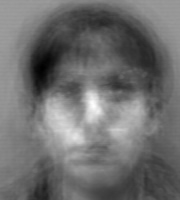
\includegraphics[width=\textwidth]{figures/rebuiltThirtySecond.png}
    \caption{A reconstruction with $s=5$.}
\end{subfigure}
\begin{subfigure}{0.32\textwidth}
    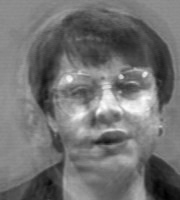
\includegraphics[width=\textwidth]{figures/rebuiltEighth.png}
    \caption{A reconstruction with $s=19$.}
\end{subfigure}
\begin{subfigure}{0.32\textwidth}
    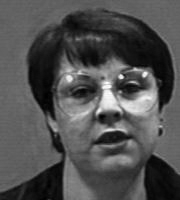
\includegraphics[width=\textwidth]{figures/rebuiltHalf.png}
    \caption{A reconstruction with $s=75$.}
\end{subfigure}
\caption{An image rebuilt with various numbers of eigenfaces. The image is already recognizable when it is reconstructed with only 19 eigenfaces---less than an eighth of the 153 eigenfaces! Note the similarities between this method and regular image compression via the truncated SVD.}
\label{fig:rebuiltImage}
\end{figure}

\begin{problem}
Instantiate a \li{FacialRec} object that draws from the \texttt{faces94} dataset.
Select one of the shifted images $\bar{\f}_i$.
For at least 4 values of $s$, use your method from Problem \ref{prob:facialrec-project} to compute the corresponding $s$-projection $\widehat{\f}_i$, then use (\ref{eq:facialrec-reconstruct}) to compute the reconstruction $\widetilde{\f}_i$.
Display the various reconstructions and the original image.
Compare your results to Figure \ref{fig:rebuiltImage}
\end{problem}

\section*{Matching Faces} % ===================================================

Let $\g$ be a vector representing an unknown face that is not part of the database.
We determine which image in the database is most like $\g$ by comparing $\widehat{\g}$ to each of the $\widehat{\f}_i$.
Fist, shift $\g$ by the mean to obtain $\bar{\g}$, then project $\bar{\g}$ using a given number of eigenfaces.
\begin{equation}
    \widehat{\g} = U_s\trp\bar{\g} = U_s\trp(\g - \boldsymbol{\mu})
    \label{eq:facialrec-unknownface}
\end{equation}

Next, determine which $\widehat{\f}_i$ is closest to $\widehat{\g}$.
Since the columns of $U_s$ are an orthonormal basis, the computation in this basis yields the same result as computing in the standard Euclidean basis would.
Then setting
\begin{equation}
j = \mathop{{\text{argmin}}\vphantom{\sim}}\limits_{\displaystyle _{i}} \|\widehat{\f}_i - \widehat{\g}\|_2, % This makes i below the argmin
\label{eq:facialrec-findnearest}
\end{equation}
we have that the $j$th face image $\f_j$ is the best match for $\g$.
Again, since $\widehat{\f}_i$ and $\widehat{\g}_i$ only have $s$ entries, the computation in (\ref{eq:facialrec-findnearest}) is much cheaper than comparing the raw $\f_i$ to $\g$.

\begin{problem} % Find nearest.
Write a method for the \li{FacialRec} class that accepts an image vector $\g$ and an integer $s$.
Use your method from Problem \ref{prob:facialrec-project} to compute $\widehat{F}$ and $\widehat{\g}$ for the given $s$, then use (\ref{eq:facialrec-findnearest}) to determine the best matching face in the database.
Return the index of the matching face.
\\(Hint: \li{scipy.linalg.norm()} and \li{np.argmin()} may be useful.)
\label{prob:facialrec-nearest}
\end{problem}

\begin{info}
This facial recognition system works by solving a \emph{nearest neighbor search}, since the goal is to find the $\f_i$ that is ``nearest'' to the input image $\g$.
Nearest neighbor searches can be performed more efficiently with the use of a \emph{$k$-d tree}, a binary search tree for storing vectors.
The system could also be called a \emph{$k$-neighbors classifier} with $k=1$.
% In this context, a $k$-neighbors classifier searches for the $k$ faces that are closest to $\g$ and use these ``neighboring'' faces to decide how to classify $\g$.
\end{info}

\begin{problem}
Write a method for the \li{FacialRec} class that accepts an flat image vector $\g$, an integer $s$, and the original dimensions of $\g$.
Use your method from Problem \ref{prob:facialrec-nearest} to find the index $j$ of the best matching face, then display the original face $\g$ alongside the best match $\f_j$.

The following generator yields random faces from \texttt{faces94} that can be used as test cases.
%
\begin{lstlisting}
def sample_faces(num_faces, path="./faces94"):
    # Get the list of possible images.
    files = []
    for (dirpath, dirnames, filenames) in walk(path):
        for fname in filenames:
            if fname[-3:]=="jpg":       # Only get jpg images.
                files.append(dirpath+"/"+fname)

    # Get a subset of the image names and yield the images one at a time.
    test_files = np.random.choice(files, num_faces, replace=False)
    for fname in test_files:
        yield np.ravel(imread(fname, flatten=True))
\end{lstlisting}
%
The \li{yield} keyword is like a \li{return} statement, but the next time the generator is called, it will resume immediately after the last \li{yield} statement.%
\footnote{See the Python Essentials lab on Profiling for more on generators.}

Use \li{sample_faces()} to get at least 5 random faces from \texttt{faces94}, and match each random face to the database with $s=38$.
Iterate through the random faces with the following syntax.
%
\begin{lstlisting}
for test_image in sample_faces(5):
    # 'test_image' is a now flattened face vector.
\end{lstlisting}
\label{prob:facialrec-match}
\end{problem}

Although there are other approaches to facial recognition that utilize more complex techniques, the method of eigenfaces remains a wonderfully simple and effective solution.

\newpage

\section*{Additional Material} % ==============================================

\subsection*{Improvements on the Facial Recognition System with Eigenfaces} % -

The \li{FacialRec} class does its job well, but it could be improved in several ways.
Here are a few ideas.
\begin{itemize}
    \item The most computationally intensive part of the algorithm is computing $\widehat{F}$.
    Instead of recomputing $\widehat{F}$ every time the method from Problem \ref{prob:facialrec-nearest} is called, store $\widehat{F}$ and $s$ as attributes the first time the method is called.
    In subsequent calls, only recompute $\widehat{F}$ if the user specifies a different value for $s$.

    \item Load a \li{scipy.spatial.KDTree} object with $\widehat{F}$ and use its \li{query()} method to compute (\ref{eq:facialrec-findnearest}).
    Building a $k$d-tree is expensive, so be sure to only build a new tree when necessary (i.e., the user specifies a new value for $s$).

    \item Include an error tolerance $\epsilon$ in the method for Problem \ref{prob:facialrec-nearest}.
    If $\|\f_j - \g\| > \epsilon$, print a message or raise an exception to indicate that there is no suitable match for $\g$ in the database.
    In this case, add $\g$ to the database for future reference.

    \item Generalize the system by turning it into a $k$-neighbors classifier.
    In the constructor, add several faces per person to the database (this requires modifying \li{get_faces()}).
    Assign each individual a unique ID so that the system knows which faces correspond to the same person.
    Modify the method from Problem \ref{prob:facialrec-nearest} so that it also accepts an integer $k$, then use \li{scipy.spatial.KDTree} to find the $k$ nearest images to $\g$.
    Choose the ID that belongs to the most nearest neighbors, then return an index that corresponds to an individual with that ID.

    In other words, choose the $k$ faces $\f_i$ that give the smallest values of $\|\f_i - \widehat{\g}\|_2$.
    These faces then get to vote on which person $\g$ belongs to.

    \item Improve the user interface of the class by modifying the method from Problem \ref{prob:facialrec-match} so that it accepts a file name to read from instead of an array.
    A few lines of code from \li{get_faces()} or \li{sample_faces()} might be helpful for this.
\end{itemize}

\subsection*{Other Methods for Facial Recognition} % --------------------------

The method of facial recognition presented here is more formally called \emph{principal component analysis (PCA) using eigenfaces}.
Several other machine learning and optimization techniques, such as linear discriminant analysis (LDA), elastic matching, dynamic link matching, and Hidden Markov Models (HMMs) have also been applied to the facial recognition problem.
Other techniques focus on getting better information about the faces in the first place, the most prevalent being 3-dimensional recognition and thermal imaging.
See \url{https://en.wikipedia.org/wiki/Facial_recognition_system} for a good survey of different approaches to the facial recognition problem.

\begin{comment}
% This proof is not needed, the Schmidt-Eckart-Young-Mirsky Theorem is sufficient to show that the first s columns of U in SVD provides the best basis for the s-dimensional subspace.
\subsection*{The Proof: SVD as a Least Squares Solution} % --------------------

\begin{theorem}
Let $\f_1, \ldots, \f_k$ be vectors in $\mathbb{R}^{mn}$, and let $\bar{F} = [\bar{f}_1 \; \ldots \; \bar{f}_k]$. Suppose $U\Sigma V\trp$ is the SVD for $\bar{F}$. Then the $s$-dimensional subspace that solves the least squares problem for $\f_1, \ldots, \f_k$ is the span of the first $s$ columns of $U$. If $U_s$ is the first $s$ columns of $U$, then the matrix $U_sU_s\trp$ is the projection onto this subspace.
\end{theorem}
\begin{proof}
We seek a rank-$s$ projection matrix $P_s$ so that $\sum_{i=1}^k \|P_s\bar{\f}_i - \bar{\f}_i\|_2^2$ is minimized---i.e.,
 the sum of the squares of the ``errors'' is minimal when we project $\bar{\f}_i$ via $P_s$.
 But minimizing this quantity is the same as minimizing its square, which happens to equal the Frobenius norm of $P_s\bar{F} - \bar{F}$.
Written mathematically,
 \begin{align*}
\inf_{\text{rank}(P_s)=s} \sum_{i=1}^k \|P_s\bar{\f}_i - \bar{\f}_i\|_2^2 &=  \inf_{\text{rank}(P_s)=s} \left( \sum_{i=1}^k \|P_s\bar{\f}_i - \bar{\f}_i\|_2^2 \right) ^2\\
 & =  \inf_{\text{rank}(P_s)=s} \| P_s\bar{F}-\bar{F}\|_F.
 \end{align*}

Now let $U \Sigma V\trp$ be an SVD of $\bar{F}$ with $\u_i$ the columns of $U$, $\v_i$ the columns of $V$, and $\sigma_i$ the singular values of $\bar{F}$.
If $P_s = \sum_{i=1}^s \u_i \u_i\trp$, then
\begin{align*}
P_s\bar{F} &=  \left( \sum_{i=1}^s \u_i \u_i\trp \right)\left(  \sum_{j=1}^k \sigma_j \u_i \v_i\trp \right)
= \sum_{i=1}^s\sum_{j=1}^k \sigma_j \u_i\u_i\trp\u_j\v_j\trp\\
&=  \sum_{i=1}^s\sum_{j=1}^k \sigma_j \u_i\delta_{ij}\v_j\trp
= \sum_{i=1}^s \sigma_i \u_i\v_i\trp.
\end{align*}

In fact, the Schmidt-Eckart-Young-Mirsky Theorem tells us that $X = \sum_{i=1}^s \sigma_i \u_i\v_i\trp$ is exactly the rank-$s$ matrix that minimizes $\|X - \bar{F}\|_F$.
Since $P_s \bar{F}$ will always have rank $s$ or less, the projection $P_s =  \sum_{i=1}^s \u_i \u_i\trp$ is the one we seek.
If we let $U_s = [ \u_1\; \ldots \; \u_s]$, then we may write $P_s = U_sU_s\trp$. Notice that $P_s$ is projection onto the subspace spanned by the columns of $U_s$.
\end{proof}

\end{comment}
